Tässä luvussa esitetään perusteet ja tarvittavat tiedot testiautomaatiosta, jotka liittyvät työn laajempaan teoreettiseen kehykseen.
Testiautomaation perusteiden ymmärtämistä tarvitaan työn myöhemmässä vaiheessa, jossa esitetään varsinainen testitapauksien priorisointi painotetun verkon avulla.

\section{Testiautomaation tarkoitus}

Testiautomaation tarkoitus on pohjimmiltaan mahdollistaa ohjelmistotuotteen jatkuva ja vaivaton laadunvarmistus, nyt ja tulevaisuudessa.
Ohjelmistojen testaamisella itsessään pyritään löytämään ohjelmistotuotteesta virheitä, anomalioita ja varmistamaan että se toimii asetettujen vaatimusten mukaisesti.
Testauksen automatisoiminen vapauttaa henkilöresursseja manuaalisesta testaamisesta muihin tuotantotehtäviin sekä parantaa toistuvien testien luotettavuutta poistamalla manuaalisessa testauksessa tapahtuvat inhimillisen virheet.
Laadunvarmistuksen osalta testiautomaatiolla voidaan kattaa erilaisia ohjelmistotuotteen laadullisia ominaisuuksia, kuten toiminnallisuus, luotettavuus, käytettävyys, tehokkuus, ylläpidettävyys ja siirrettävyys \parencite{iso_9126-1_2001}.

\section{Testauksen tasot}

Testauksen tasoja on useita ja usein ohjelmistojen kattavaan testaamiseen on suositeltavaa käyttää ohjelmistotuotantoprosessissa eri tasojen yhdistelmää.
Ohjelmistotestaus usein jaotellaan kolmeen erilaiseen menetelmään, jotka myös vaikuttavat eri testauksen tasojen käytettävyyteen.
Erilaisia menetelmiä ovat mustalaatikkotestaus, harmaalaatikkotestaus ja valkolaatikkotestaus, jotka eroavat toisistaan yleisesti ottaen siinä, otetaanko tieto ohjelmistotuotteen sisäisestä toteutuksesta mukaan testaamiseen.
Testauksen tasot voidaan jakaa neljään eri tasoon, jotka usein kuvataan pyramidin muotoon.
Pyramidimuodossa alimpana kuvataan yksikkötestaus, joka luo vahvan pohjan kokonaisvaltaiselle testaamiselle.
Noustessa pyramidissa ylöspäin testattavana olevan kohteen laajuus kasvaa.
Ylimpänä pyramidissa on hyväksymistestaus, joka on tarkoituksellista toteuttaa vaatimusmäärittelyn täyttävää valmista järjestelmää vastaan.
\begin{figure}[H]
  \centering
  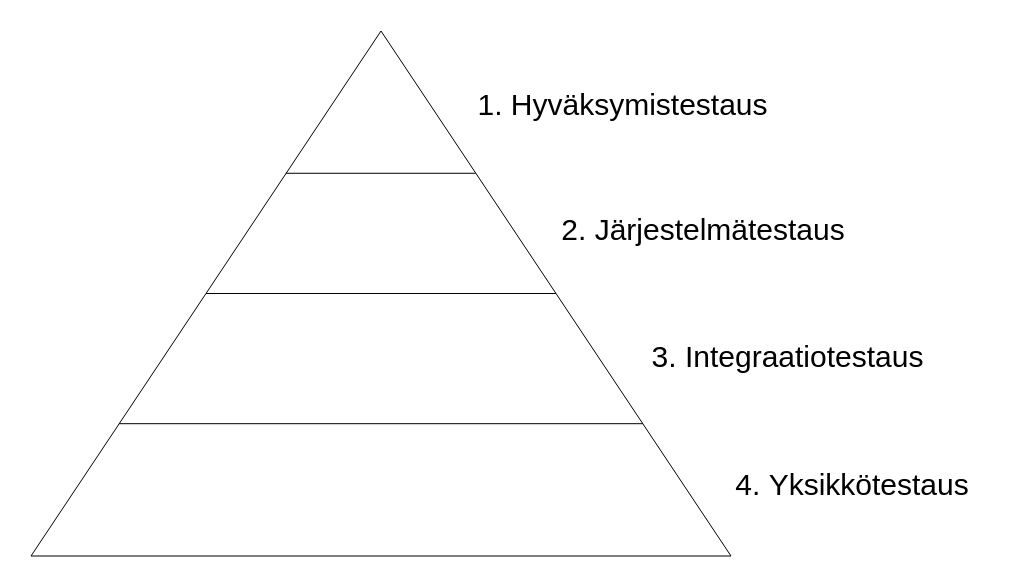
\includegraphics[width=0.8\textwidth]{assets/testing-levels-pyramid.png}
  \caption{Testauksen tasot pyramidin muodossa}
  \label{fig:testing-levels-pyramid}
\end{figure}

  \subsection{Yksikkötestaus}

  Yksikkötestauksen ajatuksena on testata ohjelmistotuotteen lähdekoodista löytyviä yksiköitä, kuten luokkia, funktioita tai moduleita.
  Yksikkötestaus toteutetaan ohjelmiston toteuttavia pienempiä yksikköjä varten.
  Yksikkötestaus eroaa muista testauksen tasoista siinä, että sen suorittavat ohjelmistokehittäjät tai ohjelmiston lähdekoodiin perehtyneet henkilöt.
  Yksikkötestauksella pyritään varmistamaan, että ohjelmiston pienimmät osat toimivat tarkoituksenmukaisella tavalla.
  Yksikkötestausta hyödynnetään usein myös ketterien menetelmien aihepiirissä, jossa ohjelmistotuotantoa toteutetaan niin sanotulla testivetoisella kehityksellä.
  Testivetoisessa kehityksessä ohjelmistokehittäjät laativat ensisijaisesti yksiköiden yksikkötestit ennen niiden toteuttamisen aloittamista.

  \subsection{Integraatiotestaus}

  Integraatiotestauksen ajatuksena on testata ohjelmistotuotteen toteuttavien eri komponenttien yhteentoimivuutta niiden rajapintojen osalta.
  Integraatiotestaus toteutetaan ohjelmiston suunnitelmaa ja mallia vastaan.
  Integraatiotestauksen onnistuminen luo perustan ohjelmiston toimimiseen ja koostamiseen kokonaisena, eri komponenteista koostuvana järjestelmänä.
  Integraatiotestauksen yhteydessä puhutaan usein myös niin sanotusta savutestauksesta, jonka tarkoituksena on koostaa päivittäinen koontiversio ohjelmistosta ja testata sen kriittisten komponenttien yhteentoimivuus.

  \subsection{Järjestelmätestaus}

  Järjestelmätestauksen ajatuksena on testata kokonaista ja toimivaa järjestelmää, yhtenä suurena yksikkönä.
  Järjestelmätestaus toteutetaan usein eräänlaisena tulikokeena, erityisesti ohjelmiston vaatimuksia vastaan.
  Järjestelmätestaukseen liittyy laajasti erilaisia testattavia laadullisia ominaisuuksia, kuten esimerkiksi toiminnallisuus, luotettavuus, käytettävyys, tietotruva, tehokkuus ja siirrettävyys.

  \subsection{Hyväksymistestaus}

  Hyväksymistestauksen ajatuksena on varmistaa toteutettavan ohjelmiston vaatimusten toimivuus erityisesti käytännön tilanteissa.
  Hyväksymistestaus toteutaan ohjelmiston toimintoja kuvaavaa vaatimusmäärittelyä vastaan.
  Hyväksymistestaus on tarkoituksenmukaista laatia sellaiseen muotoon joka testaa lopullisten käyttäjien toimintaa vastaavia käyttötilanteita.
  Samassa asiayhteydessä puhutaan usein myös niin sanotusta päästä päähän testauksesta (englanniksi: e2e, end-to-end).
  Testiautomaatio on erittäin hyödyllinen hyväksymistestausen osalla, koska sillä voidaan automatisoida ohjelmiston validointi ja hyväksyminen sekä estää puutteellisesti toimivan ohjelmiston julkaiseminen.

\section{Hyväksymistestausvetoinen kehitys}

Hyväksymistestausvetoisen kehityksen (englanniksi: ATDD, acceptance test driven development) tarkoituksena, kuten testausvetoisessakin kehityksessä on toteuttaa ohjelmistotuotannollinen prosessi testaaminen edellä.
Tämä tarkoittaa käytännössä, sitä että ohjelmistokehittäjät laativat ohjelmiston vaatimusten ja suunnitelman mukaisia iteratiivisesti suoritettavia testitapauksia, ennen niitä käyttävän varsinaisen ohjelmakoodin toteuttamista.
Hyväksymistestausvetoisessa kehityksessä luodaan ennen toteutusta tarvittavat ohjelmiston asiakasvaatimuksia palvelevat hyväksymistestit, joiden ohjelmiston on tarkoitus läpäistä.
Tarvittavat ohjelmiston hyväksymistestit suoritetaan iteratiivisesti ohjelmistokehitysprosessin aikana, ja se tarkoittaa käytännössä jatkuvan integraation ottamista käyttöön ohjelmistokehityksessä.
Hyväksysmistestausvetoinen kehitys on erittäin hyödyllinen ohjelmistokehityksessä käytetty menetelmä, sillä kehitysvaiheessa on aina tarkasti tiedossa vastaako ohjelmiston silloinen tila asiakasvaatimuksia ja kuinka hyvin.
Hyväksymistestausvetoisessa kehityksessä toteutettavat hyväksymistestit testaavat ohjelmistoa kokonaisena järjestelmänä tarkoituksenamukaisesti, siten kuten se esiintyy loppukäyttäjille.

\section{Testiautomaatio prosessina}

Testiautomaation prosessiin kuuluu erilaisia artifakteja, joita luodaan testausprosessin eri vaiheissa.
Eri vaiheita ovat kronologisessa järjestyksessä ovat muun muassa testisuunnitelma, skenaariot, testitapaukset ja seuranta.

\section{Testiautomaatio ja jatkuva integraatio}

\section{Testitapauksien määrittäminen}

Yleisiä testitapauksien määrittämiseen käytettäviä heuristiikkoja ovat muun muassa:
\begin{itemize}
  \item Polut ja tiedostot
  \item Aika ja päivämäärät
  \item Numerot
  \item Merkkijonot
  \item Yleiset rikkeet
  \item Muuttujien analyysi
  \item Kosketuspisteet
  \item Rajat
  \item CRUD-toiminnot
  \item Datan eheys
  \item Konfiguraatiot
  \item Katkokset
  \item Nälkiintyminen
  \item Samanaikaiset käyttäjät
  \item Transaktiotulvat
  \item Riippuvuudet
  \item Rajaehdot
  \item Syötetyypit
  \item Tilan analyysi
  \item Käyttäjät ja skenaariot
\end{itemize}

\section{Web-käyttöliittymien erityispiirteet}

Web-käyttöliittymillä on myös omia erityispiirteitä, jotka vaikuttavat testitapauksien laatimiseen.
\begin{itemize}
  \item Navigointi
  \item Syötteet
  \item Syntaksi
  \item Selainasetukset
\end{itemize}

\section{Priorisointiongelma}

Testitapauksien priorisointi on kustannussyistä tai resurssien optimoinnin kannalta erittäin tärkeää.
Ohjelmistotestauksessa on hyvä tiedostaa, että ohjelmistotuotetta ei usein voida testata täydellisesti, joka nostaa esiin tarpeen tärkeimpien testitapauksien löytämisestä.
Testitapauksia voidaan priorisoida monella tavalla, joihin tämä diplomityö tuo yhden uuden painottua verkkoa hyödyntävän lähestymistavan.
\begin{itemize}
  \item Painotetun verkon hyödyntäminen
  \item Muut priorisointitavat
\end{itemize}
